\documentclass[11 pt]{article}
\usepackage{amsmath, amssymb, color, xcolor}
\usepackage{graphicx, wrapfig, float, caption, dsfont, bbm}
\usepackage{fullpage}
\usepackage[backref=page, hidelinks, colorlinks=true, citecolor=blue!60!black!100]{hyperref}
\usepackage{tikz}
\usetikzlibrary{arrows.meta, shapes}
\usepackage{caption, subcaption}
\usepackage{natbib} % gives us \citet: Author (year) and \citep: (Author; year)
\usepackage{authblk}

\newcommand{\plr}[1]{{\color{blue}\it #1}}
\newcommand{\jss}[1]{{\color{olive}\it #1}}
% \newcommand{\ddt}{\frac{d}{dt}}
\newcommand{\ddt}{\dot}
\newcommand{\ro}{{ro}}
\newcommand{\nro}{{\bar{r}o}}
\newcommand{\rno}{{r\bar{o}}}
\newcommand{\nrno}{{\bar{r}\bar{o}}}
\newcommand{\reachable}{\mathcal{R}}
\newcommand{\unobservable}{\bar{\mathcal{O}}}
\newcommand{\R}{\mathbb{R}}
\newcommand{\E}{\mathbb{E}}
\renewcommand{\P}{\mathbb{P}}
\newcommand{\pda}{\frac{\partial}{\partial A_{ij}}}
\newcommand{\ind}{\mathds{1}}

\newcommand{\A}{\mathcal{A}}
\newcommand{\diag}{\text{diag}}
\newcommand{\1}{\mathbbm{1}}

\DeclareMathOperator{\spn}{span}

\newtheorem{theorem}{Theorem}
\newtheorem{lemma}{Lemma}
\newtheorem{definition}{Definition}
\newtheorem{example}{Example}

\begin{document}


\section{Introduction}

%In this paper we propose a framework to study the evolution of biological systems. To begin, we focus on the evolution of an idealized population. We consider the evolution of a perfectly adapted, large population, evolving in a static environment for an infinite number of generations. Under these ideal circumstances, we expect to observe a ``conservation of phenotype,'' where the population explores the manifold of phenotypically-invariant (or symmetric) genetic and developmental architecutres. We would like to understand which parameters influence the distribution of a population along the manifold of phenotypically invariant genetic systems. Further, we can show how dispersion along this manifold contributes to speciation and evolvability. 
\section{Notes and Ideas}

    We aim to answer the following questions and demonstrate:
      \begin{itemize}
        \item What does evolution, under phenotypic conservation, look like?
        \item How many different molecular mechanisms can realize the same phenotype? 
        \item How does evolution traverse the manifold of phenotypically identical mechanisms? 
        \item What parameters influence the qualitative aspects of neutral gene network evolution?
        \item How neutral evolution can cause speciation via reproductive isolation in F1s and F2s. 
        \item How neutral evolution influences robustness and evolvability.
        \item How these processes contribute to biological complexity (i.e. is there a ``network ratchet''? How strongly -- if at all -- does selection favor minimal molecular mechanisms?).
        \item Can we distinguish between adaptation and systems drift?
      \end{itemize}

\section{Model}
    \begin{itemize}
      \item Under the application of constant population and molecular parameters \jss{(forces?)}, such as selection, (a sufficiently large) population size, (a sufficiently small) mutation rate, stable ecology, \emph{etc.}, phenotype is invariant through evolution.
      \item Genes $\rightarrow$ Phenotype $\rightarrow$ Strategy $\rightarrow$ Fitness $\rightarrow$ Genes
    \end{itemize}

      \jss{note: add demonstration of degrees of freedom. Specifically show that if $B=C=I$ and the dimension is minimal, then there are no degrees of freedom, any $CV=C$ and $VB=B$ entails $V=I$.
      Maybe also try to do an example where speciation/hybrid incompatibility is impossible? So if the BSC concept is that, the set of high fitness GRNs is closed under the action of $V$, maybe there exits a phenotype that is also closed under averaging and recombination -- rendering incompatibility impossible -- even if very trivial it could be interesting.}

(Evolution can be described as a mapping from genes to phenotype to strategy to fitness back to genes.)

To obtain maximal fitness, an organism needs to correctly execute at least one or more of potentially an ifinite number of survival strategies. These strategies include choosing which molecule(s) to metabolize, which behavior(s) to exhibit, and which niches to compete in. Additionally, a strategy's fitness is context dependent. The organism needs to organize its phenotype in a highly specific way to play any one or more of these strategies. Presumably this is achieved by the coordinated expression of evolutionarily pliable gene networks. 
As such, we can approximately say that evolutionary fitness presupposes a termporally fluctuating set (potentially infinite) of gene-permutations with expression levels. For instance, fitness may discrimate based on an organism's ability to aquire and metabolize energy, but is ambivalent as to the source. If there are two distinct sources of energy, the combination and expression patterns of at least two (or a combination of the two) gene networks may be deemed fit. Despite this complexity, at present, we focus on the case where only one specific combination of genes and their expression levels are suitable at a time -- that is a one strategy only environment.


In this scenario, once a large population reaches a phenotype of optimal fitness, it will maintain this phenotype for infinitely long, or until a change in selection (i.e. environmental or ecological change). Here we study the null model of molecular evolution without selective flux.

    \subsection{LE Systems}
    An LE System: Linear Evolving (TI) System (in evolutionary state $\tau$), 
    \begin{align*}
      \Sigma(\tau) = \left\{ \begin{array}{cc} \dot{x} =& A(\tau)x + Bu \\
      y =& Cx \end{array} \right.
    \end{align*}
    \begin{align*}
      \mathcal{L}(\Sigma(\tau)) := H(z, \tau) = C \left(zI - A(\tau) \right)^{-1} B
    \end{align*}
    \subsection{Gene Network Diversity}
      First we need to describe the phase space. How many different gene networks can do exactly the same thing? Rather, can we describe the set of phenotypically invariant gene regulatory networks -- the set of all gene networks that produce identical outputs, when given identical inputs. In the linear case we can analytically describe all the networks in this space,
      \begin{align*}
        \mathcal{A} := \{ VAV^{-1}, CV, VB : V \in GL_{n}(\mathbb{R}) \}
      \end{align*}
      for the minimal dimension, and for the general (including non-minimal) case as,
      \begin{align*}
        CA^{k}B = \widehat{C} \widehat{A}^{k} \widehat{B} \qquad .
      \end{align*}
      where $A$ is a decription of gene network topology, and $B$ and $C$ transform the system intputs to and outputs from the network, respectively. 

  \subsection{Constant Selection Through Time}

    A large population, perfectly adapted to it's environment, under constant selection, will be phenotypically invariant for all generations (given the circumstances outlined above). Despite a conservation of phenotype, variation at the genetic and interemediate molecular levels is possible and expected through the course of evolution, as shown below. Under these constraints, phenotypic variance can only be the consequence of genetic drift (stochastic evolutionary forces overpowering selective ones due to population size) or adaptation to a novel phenotype for a different strategy (signatures of each will be discussed).

      For convenience, we hold $B$ (input transformation) and $C$ (output transformation) constant, considering only systems with varying internal mechanics.
      \begin{align*}
        P(\vec{r}) \in \{ GL_{n}(\mathbb{R}) : CP = C \text{and } BP = B \} \\
        A(\vec{r}) := P(\vec{r}) A P^{-1}(\vec{r})
      \end{align*}

      Where $A := A(0)$ be the initial and minimal configuration of a population's gene network.
      Where $\vec{r}$ is the unique vector of free variables associated with any instantiation of $P$.
      Elements of $\vec{r}$  can be restricted to a biologically reasonable range, $s \leq r_{k} \leq l$ to prevent unrealistic topologies.
      From this persepctive, the values of $A(r)$ can be written as the $n^{2}$ vector $\vec{a}(r) = \text{vec}(A(r))$. In this space, evolution acts as a random walk on $r$. 
      Furthermore, let $\Delta a(r) := \lVert \frac{d}{dr} a(r) \rVert^{-1}$. $\Delta a(r)$ describes the average magnitude of neutral genetic change required to reach a phenotypically invariant gene network. Systems should neutrally drift and rewire at rates inversely proportional to this value, as at high values of $\Delta$, more mutations are required to rewire neutrally -- that is the fitness valley is wider. Given enough time, we expect evolution to traverse the space for all of $r$, albeit at different rates and probabilities.

      Perhaps the rate of phenotypically invariant evolution near state $\tau$ can be expressed as,
      \begin{align*}
        \kappa :&= \mu \Delta_{r} = \mu \left\lVert \frac{d}{d r} \text{vec}\left[A(r)\right] \right\rVert^{-1} \\
        r &= f(\tau). 
      \end{align*}
      Where $\kappa$ is the speed the kryptotype evolves.
      \jss{Maybe need to distinguish between differentiating from the left and right of $\tau$ since we want to know the rate and direction of evolution. i.e. $\partial_{\pm} f(A(\tau))$}

      \subsection{Reproduction}
      \begin{align*}
        \text{Meiosis } &\rightarrow \begin{bmatrix} 1 & 0 \\ 0 & 0 \end{bmatrix} A_{\text{genome }1} + \begin{bmatrix} 0 & 0 \\ 0 & 1 \end{bmatrix} A_{\text{genome }2} \\
          &\rightarrow M = \text{diag}(\text{Bernoulli}(0.5)_{i}), \qquad M A_{1} + (I-M)A_{2} \\
        \text{Reproduction } &\rightarrow \frac{1}{2}(A_{\text{parent }1} + A_{\text{parent }2})
      \end{align*}
      So F1 and F2 hybrids would have the GRNs,
      \begin{align*}
        \text{F}1 &\rightarrow \frac{1}{2}(A(r) + A(\rho)) \\
        \text{F}2 &\rightarrow \frac{1}{2} \big( M A(r) + ( I - M ) A(\rho) + \widehat{M} A(r) + ( I - \widehat{M} ) A(\rho) \big)
      \end{align*}

      \subsection{Recombination -- Idea}

      Let each chromosome $\mathcal{C}$ be swapped with probability $0.5$, so the meiosis matrix $\mathcal{M}$ will have an identity matrix of appropriate dimension for each chromosome. Let intra-chromosomal recombination occur with probability $\omega \left(\gg 0.5 \right)$, breaking up the chromosomal identity matrices:
        \begin{align*}
          \mathbbm{1}_{x_{i}} &= \left\{ \begin{array}{cc} \mathcal{C}_{i} \qquad &\text{if Bernoulli}_{i}(0.5) = 1 \\ 0 \qquad &\text{if Bernoulli}_{i}(0.5) = 0 \end{array} \right. \\
            \mathcal{M} &= \begin{bmatrix} \mathbbm{1}_{x_{1}} &  & \\ & \ddots & \\ & & \mathbbm{1}_{x_{\ell}} \end{bmatrix} \\
              \mathcal{C}_{i} &= \text{diag}\left(\text{Bernoulli}\left( \omega \right) \right) \\
            A_{(\text{gamete})} &= \mathcal{M} A_{\text{genome }1} + \left(I - \mathcal{M} \right) A_{\text{genome }2}
        \end{align*}
        This formulation may be useful to see how deleterious epistatic fitness effects might not appear in a population until many generations into the future.

        After how many generations, do we expect to observe all gamete combinations. What frequency will each gamete combination occur at? 
      \subsection{Hybridization}
       F1 hybrids between $A(0)$ and $A(r)$, for the parental phenotype $H(z) = \displaystyle\frac{z-k}{\left(z-\lambda_{1}\right)\left(z-\lambda_{2}\right)}$,
      \begin{align*}
        A\left(\mathcal{H}(\, 0,r)\, \right) = \frac{1}{2} \left( A(0) + A(r) \right) = \frac{2}{(r-1)} \left[\begin{array}{cc} r\, \left(2\, \lambda_{1} - k + \lambda_{2}\right) - 2\, \lambda_{1} & - \left(k - \lambda_{2}\right)\, \left(r - 2\right)\\ \left(\lambda_{1} - k\right)\, r^2 + \left(\lambda_{2} - \lambda_{1}\right)\, r & r\, \left(k + \lambda_{2}\right) - 2\, \lambda_{2} \end{array}\right]
      \end{align*}
      F2 hybrids' gene networks are formed from the gametes of the F1s. So gametes ($G_{i}$) are formed during meiosis by swapping genes (rows) and then averaging the two new genomes in the F2 hybrid $h_{ij}$ as follows,
      \begin{align*}
        G_{1} :&= A(0) \\
        G_{2} := \text{diag}(1,0) A(0) + \text{diag}(0,1) A(r) &= \left[\begin{array}{cc} \lambda_{1} & \lambda_{2} - k\\ \lambda_{1}\, r - \frac{r\, \left(r\, \left(k - \lambda_{2}\right) + \lambda_{2}\, \left(r - 1\right)\right)}{r - 1} & \frac{r\, \left(k - \lambda_{2}\right) + \lambda_{2}\, \left(r - 1\right)}{r - 1} \end{array}\right] \\
          G_{3} := \text{diag}(0,1) A(0) + \text{diag}(1,0) A(r) &= \left[\begin{array}{cc} \lambda_{1}\, r - \frac{r\, \left(r\, \left(k - \lambda_{2}\right) + \lambda_{2}\, \left(r - 1\right)\right)}{r - 1} & \frac{r\, \left(k - \lambda_{2}\right) + \lambda_{2}\, \left(r - 1\right)}{r - 1}\\ 0 & \lambda_{2} \end{array}\right] \\
            G_{4} :&= A(r) \\
            h_{ij} :&= \frac{1}{2} \left( G_{i} + G_{j} \right)
      \end{align*}
      \jss{How does the size of a GRN contribute to hybrid incompatibility? As $n$ increases, the probability of an $A(r) \times A(r)$ cross in an F2, or even a completely $A(r)$ gamete forming during meiosis, drops rapidly.}

     \subsection{Fitness and Incompatibility}
     Hybrid Incompatibility via reproductive isolation can happen in a variety of ways. In general, if two phenotypically invariant gene networks are highly diverged such that in $A(r)$ and $A(\rho)$, $|r-\rho| \gg 0$, or if a major rewring occurs, such that in the previous example $r$ crosses from greater than to less than $1$, or vice versa, or if in special cases, the network's expression patterns are especially sensitive to perturbation. 

     However, there may be other mechanisms that lead to hybrid dysfunction. Perhaps, even a minor change in phenotype, due to negatively epistatic networks interacting, across many different networks can significantly alter a hybrid's fitness. Imagine two populations, slightly diverged, such that the first is homozygous for the $A(r)$ gene network, and the second is homozygous for the $A(r+1)$ network topology. Qualitative expression patterns in most hybrids might mirror those of the parents almost exactly -- but not quite. If the fitness cost is small, say $s=0.01$, the fitness of the hybrid would be $\Phi(h) = e^{-0.01} = 0.99$, or only $0.01$ less than each of it's parents. However, if each other hybrid gene network is equally and slightly perturbed, and the organism has $200$ networks (a lower limit estimate in humans), and fitness is multiplicitive, the fitness of a hybrid between the two populations would be $\Phi(h_{(\text{all})}) = \left( e^{-0.01} \right)^{200} \approx 0.14$, despite the fact that each individual network is only slighly less fit than the optimum. 
     \begin{align*}
        \Phi(\cdot) := \prod_{\gamma = 1}^{G} e^{-s_{\gamma}}
     \end{align*}

     Types of DMIs,
    \begin{itemize}
      \item ``parameter bifurcation'' or maybe ``rewiring'' (i.e. when $r$ jumps over $1$ in $P(r)$, as $P(r) \notin \text{GL}_{2}(\mathbb{R}$ because it is not invertible. 
      \item large neutral ``binding shifts'' or ``regulatory coefficient divergence'' when $| r - \rho | \gg 0$ for ($P(r)$ and $P(\rho)$.
      \item Dimension divergence -- If $A \in \text{GL}_{n}(\mathbb{R})$ and $\widehat{A} \in \text{GL}_{m}(\mathbb{R})$ such that $ n \neq m$.
    \end{itemize}
        These rates may be very different. If a population finds itself near its ``rewiring/bifurcation'' point $\beta$, such that $r=\beta + \varepsilon$, speciation may happen very rapidly, whereas speciation via binding shifts may take significantly more time, if possible at all, depending on the fitness function and the biological likelihood of such shitfts. For instance, $A(r)$ with respect to a theoretically possible $A(\rho)$ may exhibit a signifcant binding shift, however the coefficients set by $\rho$ may be to extreme to be realized in a biological system (\emph{e.g.} a gene regulates another greater than $\sim 10^{6}$ times the rate that itself is regulated. While these two systems may produce incomaptible hybrids, $A(\rho)$ is said to be an extremeley unlike biological manifestation of $\A$.
        Understanding the rates at which populations move in $\A$, and at which point in $\A$ gene flow was diminished among populations will allow us to predict the likelihood and rates of reproductive isolation. If $\Delta_{\tau} : \Delta_{\tau} := \mu \left\lVert \frac{d}{d \tau}\text{vec}\left[A(\tau)\right]\right\rVert^{-1}$, is very small around $r$, then binding shifts should occur rapidly. Perhaps rewiring will occur at a rate proportional to $\Delta^{2}_{\beta +\varepsilon}$ (as $\Delta_{\beta +\varepsilon} \rightarrow 0$ as $\varepsilon \downarrow 0$)?

        It may also be possible that evolution tends to favor gene networks with small regulatory coefficients. At least in the above example network, $\lVert A(r) \rVert$ is smallest as $r$ is close $\beta$. If this is the case, systems drift may be very rare, and may only/typically be due to rewiring and not shifting. Small regulatory coefficients may be favored if larger coefficients require the selective maintence of many more transcription factor binding sites in each promoter (this  may not be  a problem in populations with sufficiently small mutation rates?)?


   \section{Model Notes Version 2}

   \subsection{Evolutionarily Constant Input and Output Transformations}
    If $\Sigma_{\min}$ is a minimal system with transfer function $H(z)$, and $P$ is any invertible matrix that preserves $B$ and $C$, 
    \begin{align*}
      \Sigma_{\min} &= \{A, \ B, \ C \} \\
      P \in \mathcal{P} :&= \{ \text{GL}_{n} : PB = B, \ CP = C \text{ and } B,C \in \Sigma_{\min} \} \\
      A(\tau) \in \A :&= \{P A P^{-1} : P \in \mathcal{P} \text{ and } A \in \Sigma_{\min} \}
    \end{align*}
    $A(\tau)$ is a potential minimal gene network topology that also satisfies $H(z)$. 

    If,
    \begin{align*} 
      B \lor C^{T} = I  &\implies \\
      \mathcal{P} = \{ I \} &\implies \\
      \left\vert \A \right\vert &= 1
    \end{align*}\label{eq:k}
   then there is only one network topology of $A$ (as $\A$ only contains one element).

   Not all of the molecules and dynamics of a system, even if the system is minimal, may be directly visible to selection. As such, we distinguish between the \emph{phenotype} and the \emph{kryptotype} (\emph{pheno- ``to show''} and \emph{krypto- ``to hide''}), as selection acts directly on the phenotype molecules and only indirectly (if at all) on the molecules in the kryptotype. In \ref{eq:k} if $C=I$, the dynamics of each molecule in the system are visible to selection, and there exists only one minimal gene network organization that can precisely satisfy natural selection. It is important to note, however, that despite the uniqueness of a $A$ for the minimal case, there are an infinite number of gene network topologies with equivalent phenotypic behavior for the non-minimal case. As any gene network $\widehat{A}$ that satisfies, 
   \begin{align*}
     CA^{k}B &= \widehat{C} \widehat{A}^{k} \widehat{B} \qquad \text{for } k = 0, 1, \dots
   \end{align*}
 will be selectively indistinguishable. \footnote{If the system under study is the one in \ref{eq:k}, then for biological congruity, it probably makes sense to restrict $\widehat{B}$ and $\widehat{C}^{T}$ to the form $\left[ \begin{array}{c} I \\ \hline 0 \end{array} \right]$.} Thus in principle, under the minimal set of assumptions of this model, there are always multiple gene network topologies (and in different dimensions) that can biologically realize a given phenotype.

   To further understand neutral gene nework evolution, we need to understand how the kryptotype evolves and is contrained. Not all kryptotpes may be epistatically compatible and could lead to negative epistasis in complex traits as well as low fitness hybrids between reproducitvely isolated populations.

   \subsection{DMIs}
   Just as there are some minimal systems that cannot drift (without sacrificing fitness), there may also be systems incapable of hosting \emph{Dobzhansky-Muller Incompatibilities} (\emph{DMIs}) despite drifting.
   In the non-minimal set of systems $\A$ below,
   \begin{align*}
     H(z) :&= \frac{2}{z+3} , \ A \in \mathbb{R}^{2 \times 2}, \ C = \begin{bmatrix} 1 & 1 \end{bmatrix}, \ B = \begin{bmatrix} 1 & 1 \end{bmatrix}^{T} \\
      \A :&= \left\{ \begin{array}{cc} \left[ \begin{array}{cc} a_{11} & a_{12} \\ a_{21} & a_{22} \end{array} \right] : \begin{array}{cc} a_{11} + a_{12} &= -3 \\
   a_{21} + a_{22} &= -3 \end{array} \end{array} \right\}
   \end{align*}
   All reproductive and meiotic combinations of any element in $\A$ are also in $\A$. Thus, in the above example $\A$ is closed under recombination and reproduction. (Note: One can see that this system could easily tolerate gene duplications and evolve into an $n \times n$ system, as the phenotype is constant so long as the $n$ elements in each row sum to $-3$).

   The neutral manifold of gene network topologies for the system above is an affine, and therefore convex set. A convex set, by definition, is closed under averaging, thus any F1 hybrid among drifted networks over a convex manifold will not suffer from any incompatibilities.

   Despite the above system's immunity to negative epistasis following systems drift, many molecular systems, even minimal ones, can suffer from negative epistasis and harbor DMIs.
   For instance, the system outlined below, which oscillates in two parental populations, can be deleteriously expressed as a simple ON switch in certain F1 hybrids.

      Parental gene networks have topologies,
      $A(0) =\left[\begin{matrix}
      0 & 1 \\
      -1 & 0
    \end{matrix}\right]$
     and
    $A(2) = \left[\begin{matrix}
      2 & -1 \\
      5 & -2
    \end{matrix}\right]$ with impulse response dynamics, $f(t) = \sin(t) + \cos(t)$, can hybridize to form,
     $\mathcal{H}\left( A(0), A(2) \right) = \left[\begin{matrix}
      1 & 0 \\
      2 & -1
     \end{matrix}\right]$ which has impulse response dynamics, $f(t) = e^{t}$.


     \section{Version 3: Model Notes}

     \subsection{Outline/Premises}

      An organism is constructed by an elaborate process including complex environment-by-gene, and gene-by-gene interactions. We refer to the (heritable) characteristics of an organism that influence its chance of replication as its phenotype. In otherwords the phenotype is defined as heritable characteristics that natural selection \emph{observes} and filters. Traditionally, biologists distinguish only phenotype from genotype, however, here we will introduce (and justify the necessity of) an organism's \emph{kryptotype}. If one crudely imagines an organism to be a \emph{black box}, taking its environment as input and outputting a phenotype, its kryptotype can be thought of as the mechanism inside the blackbox as its specifics are hidden from selection. We will discuss the properties of kryptotypes, and primarily focus on the non-uniqueness and diversity of the kryptotype -- how the kryptotype can evolve and influence a myriad of evolutionary and biological phenomena such as speciation and evolvability.

     \subsection{Description of LTI and LE Systems}

     \subsection{Examples of LE Systems: kryptotype (do multiplie exist?), DMIs, Evolvability}

     \subsection{Applications to ``real'' systems: Gal Metabolism, Gap Development, Cell Cycle Control, etc.}

     \subsection{Conclusions and Future work}

     \section{Notes for May presentation}
    \begin{align*}
      \Sigma(0) := \left\{ \begin{array}{ll}
      \dot{x}_{1} &= +x_{2} + u \\
      \dot{x}_{2} &= -x_{1} + u \\
      y &= x_{1}
      \end{array} \right.
    \end{align*}
\newpage
       \begin{align*}
         \Sigma &= \left\{ \begin{array}{ll}
           \dot{\kappa}(t) &= \left[ \begin{array}{cc} 0 & 1 \\ -1 & 0 \end{array} \right] \kappa(t) + \left[ \begin{array}{c} 1 \\ 1 \end{array}\right] u(t) \\
             \phi(t) &= \left[ \begin{array}{cc} 1 & 0 \end{array} \right] \kappa(t)
         \end{array} \right. \\ \\
         \widehat{\Sigma} &= \left\{ \begin{array}{ll}
           \dot{\kappa}(t) &= \left[ \begin{array}{cc} 2 & -1 \\ 5 & -2 \end{array} \right] \kappa(t) + \left[ \begin{array}{c} 1 \\ 1 \end{array}\right] u(t) \\
             \phi(t) &= \left[ \begin{array}{cc} 1 & 0 \end{array} \right] \kappa(t)
         \end{array} \right. \\ \\
         \phi(t) &= \sin(t) + \cos(t)
        % \Sigma(2) :&= \left\{ \begin{array}{ll}
       % \dot{x}_{1} &= 2 x_{1} + - x_{2} + u \\
       % \dot{x}_{2} &= 5 x_{1} + -2 x_{2} + u \\
     % y &= x_{1}
     % \end{array} \right.
    \end{align*}
    \begin{align*}
      \mathcal{L}(\Sigma(\tau)) := H(z, \tau) = C \left(zI - A(\tau) \right)^{-1} B
    \end{align*}
    
    \begin{align*}
      f(t) &= \left( e^{\lambda_{1} t} \left(\lambda_{1} - k\right) - e^{\lambda_{2}t}\left(\lambda_{2} - k \right) \right) \frac{1}{\lambda_{1}-\lambda_{2}} \\
        H(z) &= \mathcal{L}\left(f(t)\right) \\ \\
        H(z) &= \frac{z - \lambda_{2}}{\left(z -\lambda_{1} \right)\left(z - \lambda_{2} \right)} \\
        &= C( zI - A)^{-1}B
    \end{align*}

    \begin{align*}
        H(z) &= CP^{-1}( zI - PAP^{-1})^{-1}PB \\
        &= CP^{-1}P( zI - A)^{-1}P^{-1}PB \\
        &= C( zI - A)^{-1}B \\ \\
      PB &= B \\
      CP &= C
    \end{align*}

    \begin{align*}
      P(\tau) :&= \begin{bmatrix} 1 & 0 \\ \tau & 1-\tau \end{bmatrix} \qquad \tau \neq 1 \\ \\
        A(\tau) :&= P(\tau)AP^{-1}(\tau)
    \end{align*}

    \begin{figure}
    \centering
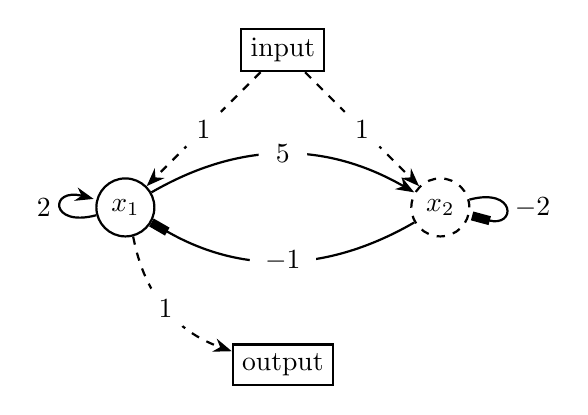
\begin{tikzpicture}
\begin{scope}[every node/.style={circle,thick,draw}]
  \node (A) at (0,0) {$x_{1}$};
    \node[dashed] (B) at (4,0) {$x_{2}$};
    \node[shape=rectangle] (U) at (2,2) {input};
    \node[shape=rectangle] (y) at (2,-2) {output};
\end{scope}

\begin{scope}[>={Stealth[black]},
              every node/.style={fill=white,circle},
              every edge/.style={draw=black, thick}]
    \path [->, sloped] (A) edge[bend left] node {$5$} (B);
    \path [->, sloped, >=Rectangle] (B) edge[bend left] node {$-1$} (A); 
    \path[->] (U) edge[dashed] node {$1$} (A);
    \path[->] (U) edge[dashed] node {$1$} (B);
    \path[->] (A) edge[dashed, bend right] node {$1$} (y);
\end{scope}
\begin{scope}[>={Stealth[black]},
              every edge/.style={draw=black, thick}]
    \path [->] (A) edge[loop left] node {$2$} (A);
    \path [->,>=Rectangle] (B) edge[loop right] node {$-2$} (B);
\end{scope}

\end{tikzpicture}
    \end{figure}

    \begin{figure}
    \centering
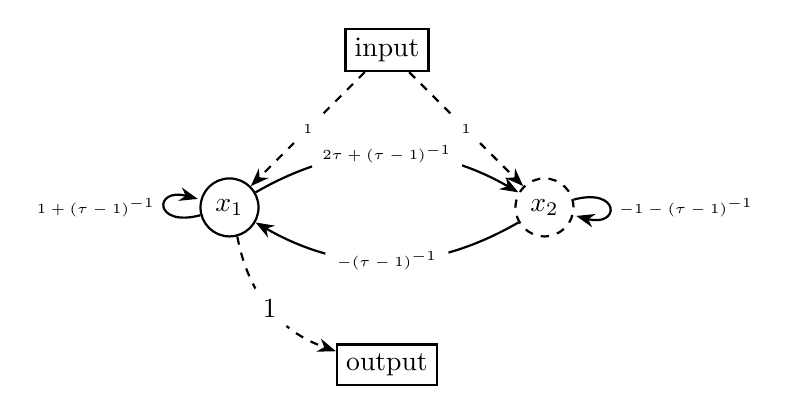
\begin{tikzpicture}
\begin{scope}[every node/.style={circle,thick,draw}]
  \node (A) at (0,0) {$x_{1}$};
    \node[dashed] (B) at (4,0) {$x_{2}$};
    \node[shape=rectangle] (U) at (2,2) {input};
    \node[shape=rectangle] (y) at (2,-2) {output};
\end{scope}

\begin{scope}[>={Stealth[black]},
              every node/.style={fill=white,circle},
              every edge/.style={draw=black, thick}]
    \path [->, sloped] (A) edge[bend left] node {\tiny $2 \tau + (\tau-1)^{-1}$} (B);
    \path [->, sloped] (B) edge[bend left] node {\tiny $-(\tau-1)^{-1}$} (A); 
    \path[->] (U) edge[dashed] node {\tiny $1$} (A);
    \path[->] (U) edge[dashed] node {\tiny $1$} (B);
    \path[->] (A) edge[dashed, bend right] node {$1$} (y);
\end{scope}
\begin{scope}[>={Stealth[black]},
              every edge/.style={draw=black, thick}]
    \path [->] (A) edge[loop left] node {\tiny $1 + (\tau-1)^{-1}$} (A);
    \path [->] (B) edge[loop right] node {\tiny $-1 - (\tau-1)^{-1}$} (B);
\end{scope}

\end{tikzpicture}
    \end{figure}
    \begin{align*}
      A(\tau) = \left[ \begin{array}{cc} \lambda_{1} - \frac{\tau \left(k-\lambda_{2}\right)}{\tau - 1} & \frac{k-\lambda_{2}}{\tau - 1} \\ \lambda_{1} \tau - \frac{\tau \left( \tau \left(k-\lambda_{2}\right) + \lambda_{2} \left(\tau-1\right)\right)}{\tau - 1} & - \frac{\lambda_{2} - k \tau}{\tau - 1} \end{array} \right]
    \end{align*}

     \begin{align*}
       \mu \Delta_{\tau} \\
       \Delta_{\tau} :&= \left\lVert \frac{d}{d \tau} \text{vec}\left[A(\tau)\right] \right\rVert^{-1} \\
      \end{align*}

      \begin{align*}
      \Delta\text{Tr} = \frac{r_{2}\left(r_{4} + r_{3} \left(\gamma-k\right)\right)}{r_{4}\left(1-r_{1}\right) + r_{2}r_{3}} 
      \end{align*}

\bibliographystyle{plainnat}
\bibliography{krefs}

\end{document}

